\documentclass{article}
\usepackage{graphicx,url}
\usepackage[brazil]{babel}
\usepackage[utf8]{inputenc}
\usepackage{enumerate}
\usepackage{tabularx}
\usepackage{multirow}
\usepackage{amsmath}
\usepackage[table,xcdraw]{xcolor}

\title{Proposta do Projeto Final \\
       da disciplina Engenharia de Softwa Experimental: \\
Ferramentas para Business Report com Suporte à Linguagem XBRL - Revisão
Sistemática da Literatura
}
\author{Vagner Clementino \\ 
       \url{vagnercs@dcc.ufmg.br}}
\date{Outubro de  2015}


\begin{document}

\maketitle

\section{Introdução}
\label{sec:intro}

O presente documento tem por objetivo descrever a proposta para o
trabalho final da disciplina Engenharia de Software Experimental. O
trabalho proposto consiste na realização de uma Revisão Sistemática da
Literatura sobre \textit{ferramentas para Business Report com suporte à linguagem XBRL}. Uma \textit{Revisão Sistemática da Literatura} - SLR (do inglês Systematic Literature Review) é uma
metodologia científica visando identificar, avaliar e interpretar
\textit{toda} pesquisa \textit{relevante} sobre um questão de pesquisa
em particular, área ou fenômeno de interesse\cite{keele2007guidelines,wohlin2012experimentation}. Business Report é processo de  divulgação
pública de informações operacionais e financeiras de uma empresa  ou a
prestação regular de informações para os tomadores de decisão dentro
de uma organização para apoiá-los em seu trabalho
\cite{lymer1999business}. Há uma terceira via do Business Report
relacionado ao processo de prestação de contas por entes públicos aos
governos nacionais. A XBRL (\textit{eXtensible Business Reporting
  Language}) é uma linguagem para divulgação e intercâmbio de
informações financeiras baseada em
XML\cite{xbrl_conceitos_aplicacoes}. O padrão vem sendo adotado por
diversas instituições e empresas em todo mundo com o suporte de um
consórcio global\footnote{\url{www.xbrl.org}} com mais de 650 membros
que incentivam a criação de jurisdições locais. Atualmente o consórcio
conta com 24 jurisdições, sendo que em países como  Estados Unidos,
Grã-Bretanha e Austrália, a XBRL já é a linguagem oficial para entrega
de relatórios à órgãos de governo. A Figura \ref{fig:world_map} exibe
os países que estão promovendo a adoção da XBRL. Estes países estão
com a coloração mais escura no mapa-múndi.

\begin{figure}[hbtp]
\centering
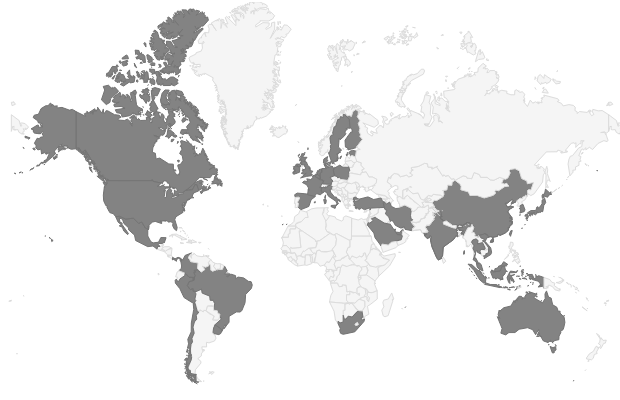
\includegraphics[width=.75\textwidth]{../img/world-map.png}
\caption{O uso da XBRL no mundo}
\label{fig:world_map}
\end{figure}

\section{Justificativa}
\label{sec:contexto}

Tendo em vista determinação da Secretaria do Tesouro Nacional, órgão
vinculado ao  Ministério da Fazenda do Brasil, que definiu o XBRL como
padrão para o envio de relatórios de prestação de contas pelos entes
federativos (estados e municípios), surge a necessidade por parte
destes últimos do \textit{desenvolvimento ou aquisição} de sistemas de
informação capazes de criar, processar e enviar informações no formato
XBRL. Um cenário onde tal situação ocorre é em pequenas ou médias
prefeituras que necessitam prestar contas via \textit{XBRL}, contudo
não possuem conhecimento ou tempo necessário para desenvolver alguma
ferramenta que suporte aquela linguagem.

Neste sentido,  verifica-se que existe a necessidade por parte das
organizações, especialmente as entidades públicas, de referências de
qualidade sobre o assunto de \textit{XBRL}. Neste contexto, entende-se que uma Revisão Sistemática da
  Literatura - SLR  que avaliasse as ferramentas para Business Report que dão suporte ao
XBRL pode \textit{subsidiar a tomada de decisão} por parte dos gestores
públicos sobre a aquisição de tais ferramentas. Além de dar suporte à
tomada de decisão um trabalho neste sentido poderia subsidiar o
desenvolvimento de novas ferramentas que venham preencher as eventuais
lacunas que por ventura os sistemas atuais tenham deixado. Ademais,
traz o foco da comunidade científica sobre um assunto que não é tão
novo, todavia, vêm crescendo bastante nos últimos anos pela
necessidade das organizações de serem cada vez mais transparentes. 

\section{Objetivos do Trabalho}
\label{sec:objetivos}

O trabalho ora proposto tem como objetivo desenvolver dois trabalhos
empíricos sobre o assunto \textit{XBRL}. A primeira parte consiste no
desenvolvimento de uma \textit{Revisão Sistemática da Literatura -
  SLR} sobre ferramentas de \textit{Business Report} com suporte ao
padrão XBRL. O público alvo do referido trabalho serão pesquisadores,
programadores, gestores que precisam de uma fonte de informação
independente que avaliasse as soluções existentes no mercado. A partir
dos dados obtidos da \textit{SLR} seria possível, por exemplo, propor
novas Ferramentas ou mesmo melhorias nas existentes.

\section{Estudo Preliminar}
\label{sec:rsl}

Uma Revisão Sistemática da literatura (SLR), por se tratar de método
científico, deve seguir uma sequência rigorosa de passos a fim de
alcançar os seus objetivos. Alguns diretrizes orientam como sequências
fundamentais no processo de desenvolvimento de uma
SLR\cite{keele2007guidelines}, dentre outras: 
\begin{itemize}
  \item especificar uma ou mais sentenças de buscas que serão
    inseridas nas ferramentas de busca com o objetivo de recuperar os
    estudo preliminares que serão utilizados na revisão;
  \item definir um conjunto de \textit{questões de pesquisa} que
    servirão de norte na condução do trabalho;
 \item  desenvolver um protocolo que definirá os procedimentos a serem adotados durante a revisão, ele servirá como um guia para a condução da revisão. 
\end{itemize}

Nas próximas subseções iremos detalhar cada um dos passos descrito anteriormente.
\subsection{Sentenças de Busca}
\label{subsec:setences}

Como a revisão proposta tem como principal objetivo ser uma referência para aqueles interessados em avaliar ferramentas de Business Report com suporte à XBRL, naturalmente sentenças como ``XBRL", ``tools", ``Business Report"\footnote{Inicialmente será utilizado apenas as sentenças na língua inglesa} se mostram como boas candidatas. 

A fim de avaliar qual sentença de busca possibilitaria um conjunto de
estudos preliminares com maior relevância para o trabalho, foi
realizada um estudo prévio utilizando a ferramenta de pesquisa Google
Schoolar\footnote{\url{https://scholar.google.com.br/}}. O estudo é
bastante simples, consistindo apenas em registrar o total de artigos
recuperados quando realizado uma pesquisa com uma sentença $S_n$
qualquer. Não foi utilizado qualquer tipo de filtro na busca (como por
exemplo "por data") e os resultados foram classificados por
relevância. Apesar do simplicidade deste estudo ele se mostra como um
bom ponto de partida para definirmos a sentenças de buscam que
futuramente irão possibilitar a recuperação dos estudos preliminares. A tabela \ref{tab:sentencas} exibe as sentenças utilizadas bem como o total de artigos recuperados.


\begin{table}[]
\centering
\resizebox{\textwidth}{!}{%
\begin{tabular}{clc}
\rowcolor[HTML]{EFEFEF} 
{\bf Código da Sentença} & \multicolumn{1}{c}{\cellcolor[HTML]{EFEFEF}{\bf Sentença}} & {\bf Total de Artigos}     \\ \hline
\multicolumn{1}{|c|}{$S_1$} & \multicolumn{1}{l|}{“XBRL”}                                & \multicolumn{1}{c|}{15000} \\ \hline
\multicolumn{1}{|c|}{$S_2$} & \multicolumn{1}{l|}{“XBRL tools”}                          & \multicolumn{1}{c|}{3710}  \\ \hline
\multicolumn{1}{|c|}{$S_3$} & \multicolumn{1}{l|}{“XBRL Business Report tools”}          & \multicolumn{1}{c|}{4110}  \\ \hline
\multicolumn{1}{|c|}{$S_4$} & \multicolumn{1}{l|}{“XBRL tools marketing”}                & \multicolumn{1}{c|}{1290}  \\ \hline
\multicolumn{1}{|c|}{$S_5$} & \multicolumn{1}{l|}{“XBRL Business Report software tools”} & \multicolumn{1}{c|}{2970}  \\ \hline
\end{tabular}
}
\caption{Total de artigos por sentença}
\label{tab:sentencas}
\end{table}

Como pode ser observado a sentença $S_1$ é a consulta mais genérica que poderia ser feita sobre no contexto da XBRL, contudo, é retornado um total de $15000$ um valor relativamente pequeno comparado ao total de artigos retornados ao realizar consultas com o termo ``XML' por exemplo\footnote{A consulta por XML retorna aproximadamente $3 \times 10^{6}$ artigos}.

Não obstante a sentença $S_6$ se mostrou satisfatória tanto pelo total
de artigos recuperados bem como pela relevância dos mesmo, auferida
pela inspeção manual de alguns resultados. Visando avaliar o impacto
de restringir o ano de publicação na sentença $S_6$ foi realizada um
novo conjunto de buscas no qual foi utilizado o critério de seleção
``artigos a parte do ano''.  Os resultados são exibidos na Figura \ref{fig:graph_artigos_ano}{}.

\begin{figure}[h] 
\label{fig:graph_artigos_ano}
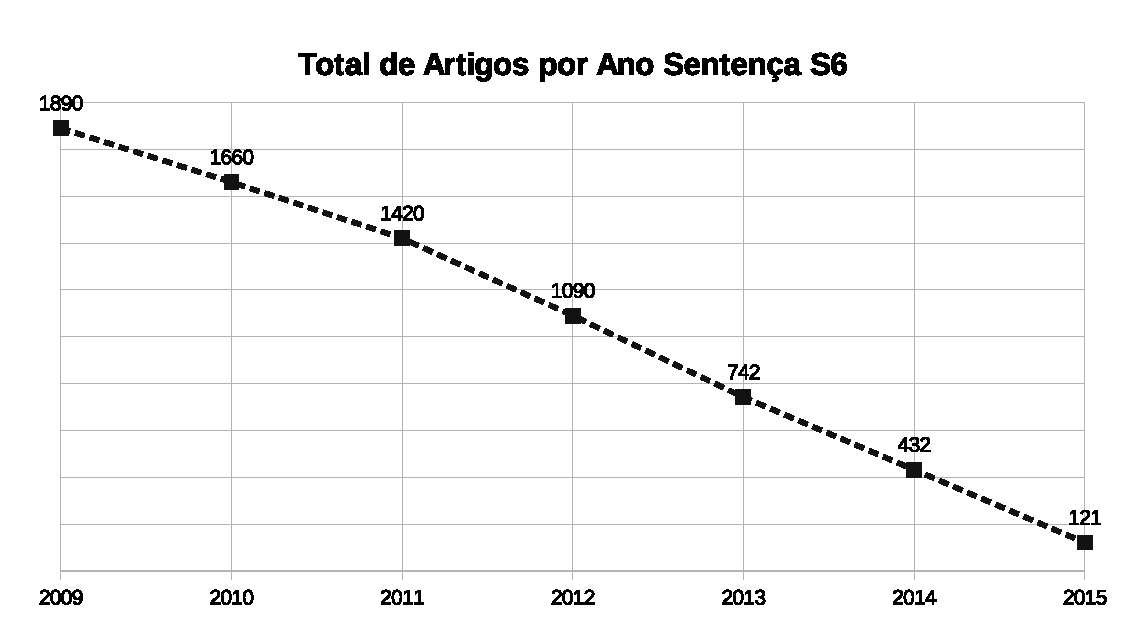
\includegraphics[width=8cm]{../img/graph_01.eps}
\caption{Total de artigo a partir de determinado ano para a sentença $S_6$}
\centering
\end{figure}

A Figura \ref{fig:graph_artigos_ano} mostra conforme esperado a
redução do número de artigos quanto se limita o período de
pesquisa. Em uma análise preliminar pode-se afirmar que a utilização
de artigos publicados a partir de 2012 consegue englobar uma massa de
artigos suficiente para um estudo ponto de partida. Posteriormente,
mediante o Protocolo da Revisão serão definidos critérios para
inclusão e exclusão de ababalho na revisão. Os detalhes destas
diretrizes estão detalhadas na Subseção \ref{subsec:protocol}.

\subsection{Questões de Pesquisa}
\label{subsec:research_question}

In work.

\subsection{Protocolo de Desenvolvimento da Revisão}
\label{subsec:protocol}

Aguardando definições.

\section{Survey com Stakeholders}
\label{sec:survey}

Avaliando viabilidade.

\section{Cronograma}
\label{sec:cronograma}


\section{Próximas Etapas}
\label{sec:proximas_etapas}

Aguardando definições.

\medskip

\bibliographystyle{unsrt}%Used BibTeX style is unsrt
\bibliography{../bib/propostaref}

\end{document}
